\section{Introduction}
Hyperboloidal slices place future null infinity at a finite coordinate location while retaining a spacelike initial-value surface. They therefore offer direct access to outgoing radiation, but conformal compactification introduces formally singular coefficients into free-evolution equations. Spherical calculations have established that gauge choices and constraint damping are central to obtaining regular numerical evolutions\cite{VHH2015,VH2014,VH2018}. Black-hole trumpet constructions, dynamical conformal diagrams, and alternative reference metrics provide complementary tests of the same asymptotic difficulty\cite{VV2023,VV2024,VVValente2024}.

The present experiment replaces a hyperbolic shift driver by a condition on the \emph{metric-derived} reference connection. The distinction matters: freezing a connection computed from the metric need not suppress an independently evolved connection constraint. Our aim is to retain free Z4c evolution while controlling conformal metric shape through an elliptic gauge solve. The supplied linearized closure notes motivate this construction, but concern a compatible perturbative phase around hyperboloidal Minkowski spacetime. They do not establish nonlinear black-hole or Einstein--scalar stability.

This paper reports the evidence presently available, including unsuccessful variants. Its principal new strong-field result is a full-domain, three-grid telegrapher lapse study through $t=10$, which passes the declared spatial checks while retaining a narrow inner lapse feature and strong characteristic compression. This result complements implementation checks, weak-field convergence, and coupled subcritical mass--flux tests; it does not establish long-time nonlinear stability. The failed pre-telegrapher front is preserved in Appendix~\ref{app:pre-telegrapher}. The different experiments use explicitly labeled gauge and numerical variants; they do not constitute a single universally successful parameter choice. We distinguish an exact identity, agreement between implementations, convergence of a numerical experiment, and successful completion of a physical scenario throughout.

\section{Nonlinear spherical formulation}
\label{sec:formulation}
\subsection{Fields and conventions}
We set $G=c=1$ and use the compactification length as the unit of length and time. The fixed conformal factor and Minkowski reference are
\begin{equation}
 \begin{gathered}
 \Omega=(1-r^2)/2,\qquad A=(1+r^2)/2,\\
 \beta_\star=-r,\qquad K_\star=-3.
 \end{gathered}
\label{eq:reference}
\end{equation}
The outer boundary is the actual grid point $r=1$ at $\Iplus$. The physical metric is $\widetilde g_{ab}=\Omega^{-2}\bar g_{ab}$, with conformal lapse $\alpha$, radial shift $\beta$, and spatial line element
\begin{equation}
 \dd\widetilde\ell^2=\frac{1}{\Omega^2\chi}
 \left[g\,\dd r^2+r^2g^{-1/2}\dd\omega^2\right].
\label{eq:metric}
\end{equation}
The physical lapse is $\widetilde\alpha=\alpha/\Omega$. The freely evolved geometric fields are
\begin{equation}
 (\chi,g,\Ar,\Kh,\Th,\Lambda^r,\alpha),\qquad
 \Kh=K-2\Th,
\end{equation}
where $K$ and $\Th$ have physical normalization and $\Ar=A_{rr}$ is the conformal radial trace-free curvature variable, normalized so that $K^r{}_r-K/3=\Omega\Ar/g$. The angular metric and curvature components follow from the algebraic determinant and trace conditions. These algebraic reductions do not solve the Hamiltonian or momentum constraints.

The spherical restriction retains angular tensor derivatives. For example, the transverse Hessian of a radial scalar is $f_r/r$; vector and tensor derivatives contain additional angular terms. A native tensor implementation constructs these derivatives explicitly and supplies an independent comparison for the canceled radial implementation. Most evolution results use initially isotropic conformal data, $g=1$, for which the metric-freezing gauge preserves $g=1$. Appendix~\ref{app:equations} gives the corresponding nonlinear vacuum equations and constraints. The remaining curvature, trace, and Z4 variables stay independent.

\subsection{Metric-derived elliptic shift}
Let $V^r$ denote the contracted connection difference computed from the conformal metric and the flat spherical reference connection. Direct contraction gives
\begin{equation}
 V^r=\frac{g_r}{g^2}+\frac{2}{r}\left(\sqrt g-\frac1g\right),
 \qquad Z_r=\frac g2(\Lambda^r-V^r).
\label{eq:V}
\end{equation}
In particular, $V^r$ and $\Lambda^r$ are different quantities off the constraint surface. Write the radial metric rate as
\begin{equation}
 Q\equiv\partial_tg=\beta g_r+\frac{4g}{3}
 \left(\beta_r-\frac\beta r\right)-2\alpha\Ar.
\end{equation}
Differentiating Eq.~\eqref{eq:V} yields
\begin{equation}
 \partial_tV^r=\frac{1}{g^2}(Q_r+P_g Q),\qquad
 P_g=-\frac{2g_r}{g}+\frac{g^{3/2}+2}{r}.
\end{equation}
The gauge $\partial_tV^r=-\eta_D V^r$, with $\eta_D\geq0$, is therefore a second-order radial equation for $\beta$. With $C_g=4g/3$ and $D_g=g_r-4g/(3r)$, it reads
\begin{align}
 C_g\beta_{rr}+(C_{g,r}+D_g+P_gC_g)\beta_r
 &+(D_{g,r}+P_gD_g)\beta \nonumber\\
 =2(\alpha\Ar)_r+2P_g\alpha\Ar&-\eta_Dg^2V^r.
\label{eq:elliptic}
\end{align}
Its principal coefficient is positive for $g>0$.

For $g=1$ and metric freezing, the homogeneous metric-rate equation is $Q_r+3Q/r=0$. Center regularity excludes $Q\propto r^{-3}$, leaving $Q=0$. The analogous bounded-shape condition excludes this mode at the asymptotically flat inner end. Defining $W=(\beta+r)/r$, one obtains
\begin{align}
 W_r&=\frac{3\alpha\Ar}{2r},\label{eq:W}\\
 W(1)&=-\frac{c+(2u+u^2)\chi}{1+\alpha\sqrt\chi}\bigg|_{r=1},\nonumber
\end{align}
where $c=\chi-1$ and $u=\alpha-A$.
The boundary value is an algebraically stable form of the null-normal shift condition. It fixes the remaining homogeneous shift mode. Thus $\beta$ is determined without using $\Lambda^r$, $\HH$, or $\MM$. At a later finite cutoff, $Q=0$ is retained as an explicit inherited elliptic gauge condition; the regular-center uniqueness argument is not reapplied to that truncated domain.

\subsection{Live lapse and disclosed source variants}
With $v=\beta+r$ and $p=\Kh$, the baseline lapse equation is
\begin{align}
 \partial_t\alpha={}&\beta u_r+rv+\frac{S_\alpha}{\Omega},\nonumber\\
 S_\alpha={}&-F(p+3)+r(Av-ru+uv)-\mathcal D,\label{eq:lapse}\\
 F={}&\alpha^2+4\nu\Omega^2\alpha.\nonumber
\end{align}
The term proportional to $\alpha$ gives logarithmic-slicing-like behavior in the interior, whereas $F\to\alpha^2$ at scri. This is not exact physical $1+\log$ slicing at every interior point. The pulse experiments use $\nu=1$ and symmetric restoring,
\begin{equation}
 \mathcal D_{\rm sym}=\xi(\alpha+A)(\alpha-A),\qquad\xi=1.
\end{equation}
This restoring term is an explicit gauge modification relative to the original un-restored reference prescription.

The same untapered symmetric source obstructs a regular stationary collapsed lapse at a puncture. If $\alpha\sim r^\gamma$, $\gamma>0$, $\beta=O(r)$, and $\Kh$ stays finite, the other lapse terms vanish at $r=0$, but
\begin{equation}
 \partial_t\alpha(0)=\frac{\xi}{2}.
\label{eq:obstruction}
\end{equation}
This conditional statement concerns that source choice, not free Z4c or elliptic shifts in general. A multiplicative control,
\begin{equation}
 \mathcal D_{\rm mult}=2\xi\alpha(\alpha-A),
\end{equation}
removes the constant and differs from the symmetric lapse numerator by $-\xi u^2$. It preserves the linearization about Minkowski, but does not by itself provide stable black-hole evolution.

The later wormhole tests also use
\begin{align}
 \xi_{\rm eff}(r)&=\xi+(3\nu-\xi)(2\Omega)^4,\nonumber\\
 \Delta S_\alpha&=(2\Omega)^4r^2\frac{\alpha-A}{A},
\label{eq:physical-log}
\end{align}
with multiplicative restoring. These changes preserve the Minkowski equilibrium and the leading scri limits, but \emph{change the interior linearized gauge}. We refer to this as the modified logarithmic source. The main black-hole tests retain the Minkowski lapse reference. A distinct already-trumpet control adds an analytic CMC lapse source; it is identified separately in Sec.~\ref{sec:cmc}.

\subsection{Off-constraint terms}
The candidate uses $\kappa_1=4$, $\kappa_2=-0.99$. The scalar-$\Th$ equation differs from the repository control by
\begin{equation}
 \Delta(\partial_t\Th)=\frac{3\alpha w\Th}{\Omega},\qquad
 w=\bar n(\Omega)=\frac{\beta r}{\alpha}.
\label{eq:theta-change}
\end{equation}
This removes a repository $-3\alpha w\Th/\Omega$ term and implements the tested Appendix-C-style choice\cite{VHH2015}. The change vanishes on the constraint surface, but changes the off-constraint system. Agreement with the native implementation alone does not constitute a complete independent audit of every published Appendix C term.

A separate reference-lapse damping control replaces products $\alpha\kappa_1$ by $A\kappa_1$. The implementation evaluates those products directly, avoiding division by a collapsed lapse. This changes damping away from the constraint surface. We do not combine results from this control with constant-damping experiments as if they used identical equations.

\begin{figure*}[tp]
 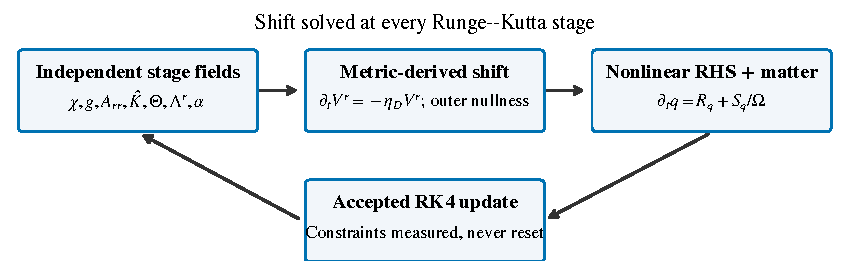
\includegraphics[width=\textwidth]{scheme}
 \caption{Stage structure of the method. The elliptic equation controls the metric connection, while $\Lambda^r$, $\Th$, curvature, and the trace remain evolved fields. The diagram describes the algorithm, not a stability theorem. Scalar sources and radiation flux, when present, are evaluated at the same RK stages.}
 \label{fig:scheme}
\end{figure*}
